\chapter{Modelado de un cuadricóptero}

Un cuadricóptero es un robot aéreo con 6 grados de libertad (3 rotacionales y 3 traslacionales) y 4 motores, al tener menos motores que el número de grados de libertad, se dice que es un sistema subactuado.

\begin{figure}[htb!]
	\centering
	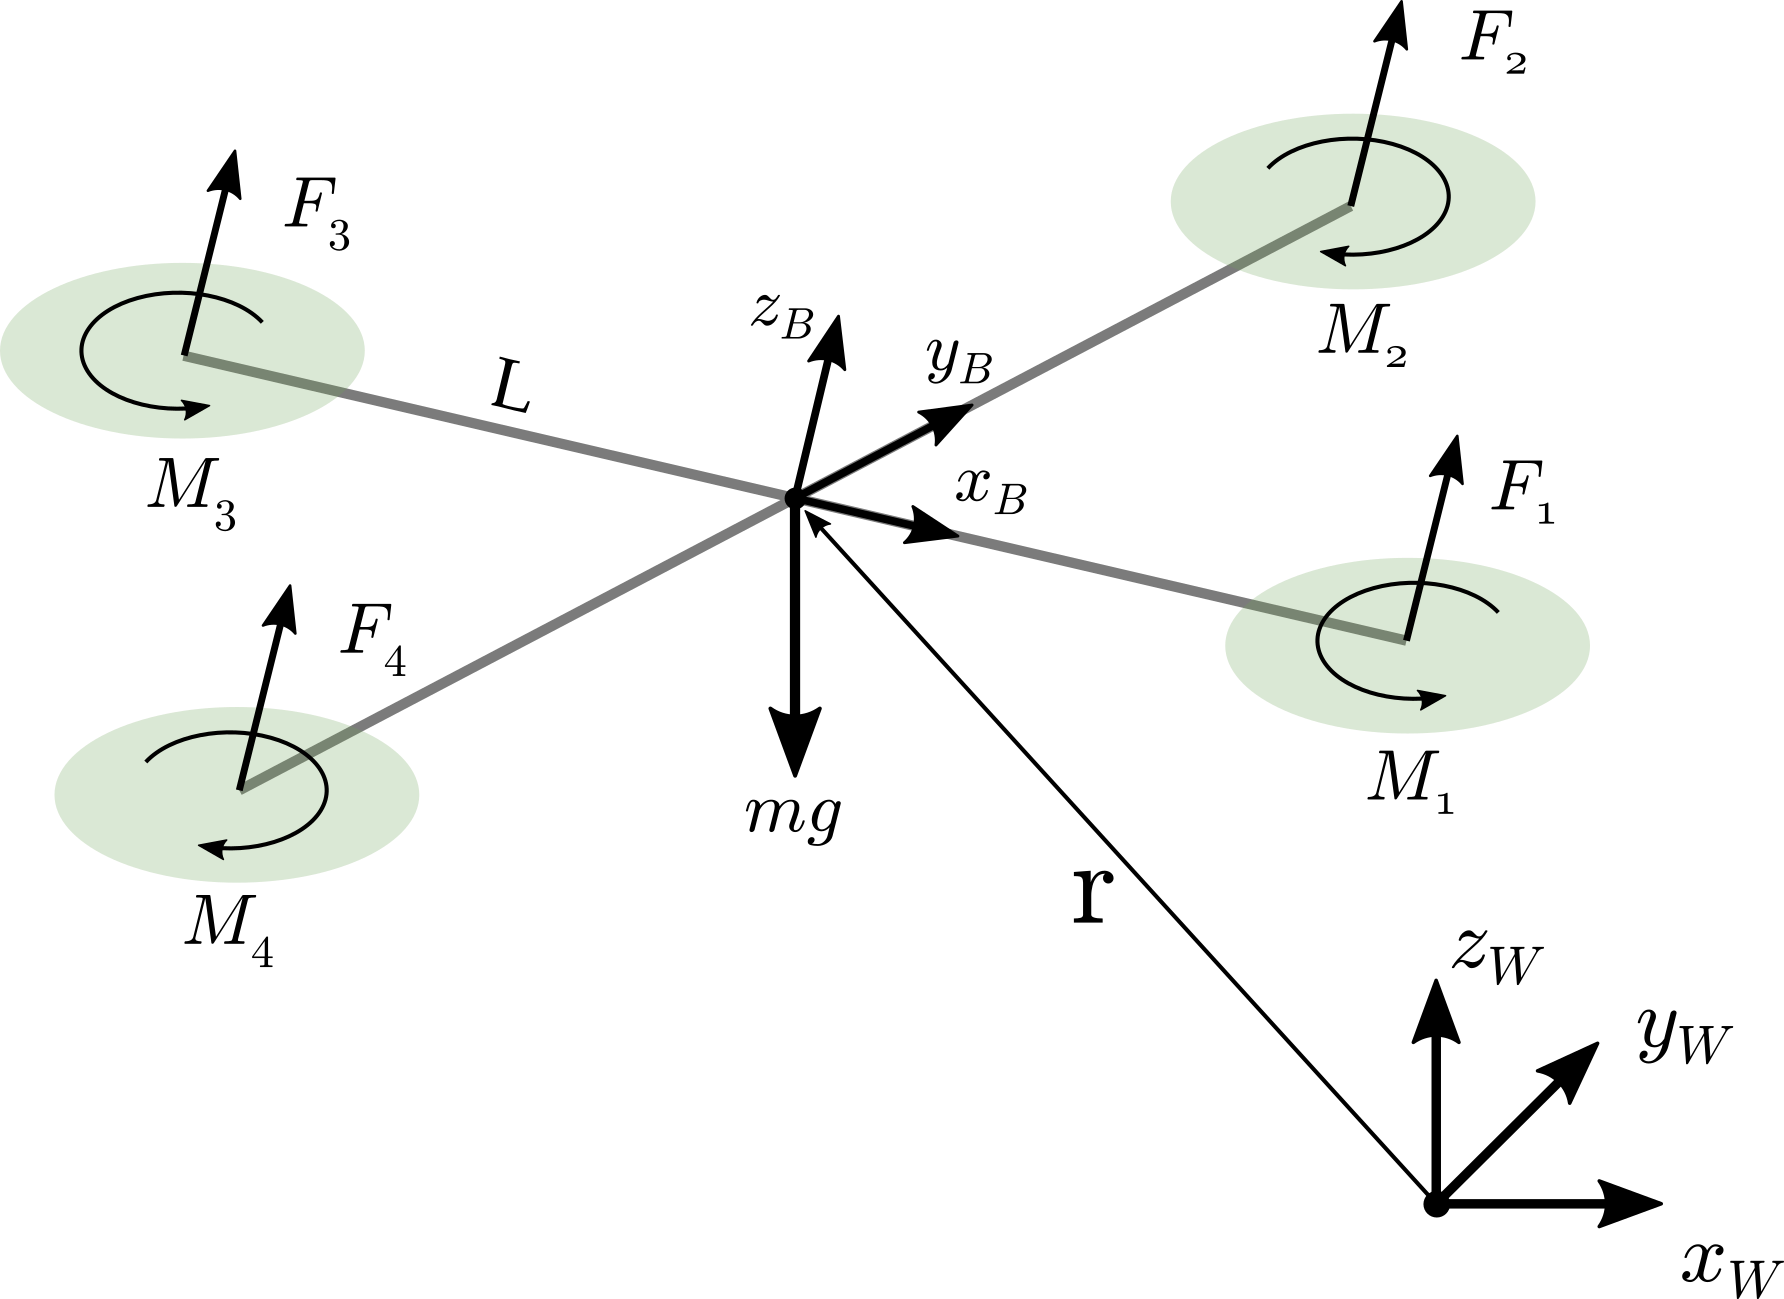
\includegraphics[width=0.65\textwidth]{imagenes/uav_coordinate_system}
	\caption{Esquema de fuerzas y momentos que actúan sobre un cuadricóptero y sus sistemas de referencia asociados. }
	\label{modelado:uav_coordinate}
\end{figure}

Como puede observar en la figura \ref{modelado:uav_coordinate}, se ha  empleado el subíndice $W$ para hacer referencia al sistema de referencia del mundo, así como el subíndice $B$ para referirse al sistema asociado al cuerpo del cuadricóptero. El \textit{frame} $B$ posee su origen $O_B$ en el centro de masas de la aeronave, con el eje $x_B$ coincidente con la dirección de avance preferente de la aeronave.

Para modelar las rotaciones del \textit{frame} $B$ con respecto a $W$ se emplearán los ángulos de Euler Z-X-Y, es decir, la matriz de rotación $R$ para transformar coordenadas desde $B$ a $W$ consiste en la composición de las siguientes rotaciones:
\begin{equation}
	R = R_{\mathbf{z},\psi}R_{\mathbf{x},\phi}R_{\mathbf{y},\theta}
	\label{modelado:euler_z_x_y}
\end{equation}
siendo $R_{\mathbf{i},\alpha}$ una rotación de un ángulo $\alpha$ respecto al eje $i$. Al desarrollar la expresión \ref{modelado:euler_z_x_y} se obtiene la matriz $R$ resultante
\begin{equation}
	\label{modelado:R}
	R = \begin{bmatrix}
		c_{\psi} c_{\theta} - s_{\phi} s_{\psi} s_{\theta} &  -c_{\phi} s_{\psi}& c_{\psi} s_{\theta} +  c_{\theta} s_{\phi} s_{\psi}\\
		c_{\theta} s_{\psi} +  c_{\psi} s_{\phi} s_{\theta} & c_{\phi} c_{\psi} & s_{\psi} s_{\theta} -  c_{\theta} s_{\phi} c_{\psi} \\
		-c_{\phi}s_{\theta}& s_{\phi} & c_{\phi}c_{\theta} 
	\end{bmatrix}
\end{equation}

donde $c_{\theta}$ y $s_{\theta}$ denotan $cos(\theta)$ y $sen(\theta)$ respectivamente.

En el sistema de referencia $B$ las componentes del vector velocidad angular $\Omega$ están definidas por $p$, $q$ y $r$ de la forma: 

\begin{equation}
	\Omega = p \mathbf{x_B} + q \mathbf{y_B} + r \mathbf{z_B}
\end{equation}

Estas componentes están relacionadas con las derivadas de los ángulos de Euler de acuerdo a

\begin{equation}
	\begin{bmatrix}
		p\\
		q\\
		r
	\end{bmatrix}  = \begin{bmatrix}
	c_{\theta}&0& -c_{\phi} s_{\theta}\\
	0 & 1 & s_{\phi}\\
	s_{\theta}&0 & c_{\phi} c_{\theta}
\end{bmatrix}\begin{bmatrix}
\dot{\phi}\\
\dot{\theta}\\
\dot{\psi}
\end{bmatrix} 
\end{equation}

\section{Análisis dinámico}
\subsection{Ecuaciones de movimiento traslacional}
Como se puede observar en la figura \ref{modelado:uav_coordinate}, las fuerzas que actúan sobre el cuadricóptero son: la gravedad, en la dirección $-\mathbf{z_W}$ y la fuerza de cada uno de los motores, en la dirección $\mathbf{z_B}$. Para hallar las ecuaciones que rigen la dinámica del centro de masas del sistema $C$ se aplican las ecuaciones de Newton sobre él. Siendo $\mathbf{r}$ el vector de posición del centro de masas $C$ con respecto al origen de $W$ obtenemos:

\begin{equation}
	\label{analisis:eq1}
	m \mathbf{\ddot{r}} = \begin{bmatrix}
		0\\
		0\\
		-mg
	\end{bmatrix} + R \begin{bmatrix}
	0\\
	0\\
	F_1+F_2 + F_3 + F_4
\end{bmatrix}
\end{equation}

Si denominamos $F  = \displaystyle\sum_{i=1}^{4}F_i$ , al expandir la ecuación anterior con la definición de $R$ en \ref{modelado:R} obtenemos las ecuaciones que describen el movimiento traslacional del centro de masas del cuadricóptero:

\begin{equation}
	\label{analisis:eq2}
	m \mathbf{\ddot{r}} = \begin{bmatrix}
		0\\
		0\\
		-mg
	\end{bmatrix} +\begin{bmatrix}
		s_{\theta}c_{\psi} + s_{\phi}c_{\theta}s_{\psi} \\
		s_{\theta}s_{\psi} - s_{\phi}c_{\theta}c_{\psi} \\
		c_{\phi}c_{\theta}
	\end{bmatrix} F
\end{equation}

\subsection{Ecuaciones de movimiento rotacional}

Como se puede observar en la expresión anterior, el movimiento del cuadricóptero depende de la rotación $R$, por lo que es necesario modelar el movimiento rotacional del mismo. Se define el momento angular $H$ como:
\begin{equation}
	H = \mathbf{I}\Omega
\end{equation}
donde $\mathbf{I} \in \mathbb{R}^{3\times 3}$ representa el tensor de inercia del cuadricóptero en el sistema $B$, y $\Omega  = [p, q, r]$ representa el vector de velocidad angular de $B$ respecto $W$. 

Si denotamos $M_c = [\tau_x, \tau_y, \tau_z]^t$ como el momento total del cuadricóptero en el sistema $B$

\begin{align}
	M_c &= \frac{d}{dt}H\nonumber\\
		&= \mathbf{I}\dot{\Omega}+\Omega\times\mathbf{I}\Omega
	\label{model:rot1}
\end{align}

Se considera que el cuadricóptero presenta una distribución de masa simétrica, por lo que el tensor de inercia $\mathbf{I}$ es un tensor diagonal de la forma:

\begin{equation}
	\mathbf{I} = \begin{bmatrix}
		I_{xx}&0&0\\
		0&I_{yy}&0\\
		0&0&I_{zz}\\
	\end{bmatrix}
\end{equation}
siendo $I_{xx}$, $I_{yy}$, $I_{zz}$ los momentos principales del cuadrícoptero con respecto a los ejes $x_B$, $y_B$, $z_B$ respectivamente.

Desarrollando la expresión \ref{model:rot1} y reorganizando sus términos:
\begin{align}
\mathbf{I}\begin{bmatrix}
	\dot{p}\\
	\dot{q}\\
	\dot{r}
\end{bmatrix}=
\begin{bmatrix}
	\tau_x\\
	\tau_y\\
	\tau_z
\end{bmatrix} -\begin{bmatrix}
	p\\
	q\\
	r
\end{bmatrix} \times\mathbf{I}\begin{bmatrix}
	p\\
	q\\
	r
\end{bmatrix}\label{model:rot2}
\end{align}

A partir del diagrama de la figura \ref{modelado:uav_coordinate} se puede calcular los valores de $\tau_x$, $\tau_y$ y $\tau_z$ a partir de las fuerzas y momentos ejercidos por los motores.

\begin{align}
	\tau_x &=  L (F_2-F_4)\nonumber\\
	\tau_y &=  L (F_3-F_1)\nonumber\\
	\tau_z &=  M_1 - M_2 + M_3 - M_4\label{model:rot3}
\end{align}

Finalmente se unen las expresiones \ref{model:rot2} y \ref{model:rot3} para obtener la ecuación de movimiento rotacional del cuadricóptero.






\begin{align}
	\mathbf{I}\begin{bmatrix}
		\dot{p}\\
		\dot{q}\\
		\dot{r}
	\end{bmatrix}=
	\begin{bmatrix}
		L (F_2-F_4)\\
		L (F_3-F_1)\\
		M_1 - M_2 + M_3 - M_4
	\end{bmatrix} -\begin{bmatrix}
		p\\
		q\\
		r
	\end{bmatrix} \times\mathbf{I}\begin{bmatrix}
		p\\
		q\\
		r
	\end{bmatrix}
\end{align}





\chapter{Control}


El problema del control se puede expresar formalmente: 
Dado el estado del sistema $x(t)$ \tb{continuar . ... }
como encontrar la función $u(t)$ tal que, el estado $x(t)$ sigue la trayectoria desesada $x^{des}(t)$ a lo largo del tiempo.\\
Si se define el error $e(t)$ del control como:
\begin{equation}
	e(t) = x^{des}(t) - x(t)
\end{equation}
el objetivo del controlador sería conseguir que el error $e(t)$ converja de forma exponencial a 0.


El estado $x(t)$ de un cuadricóptero consta de 12 variables, las 6 correspondientes a su pose y sus derivadas correspondientes.
\begin{equation}
	x(t) = \left[
	x  \;\;
	y  \;\;
	z  \;\;
	\phi  \;\;
	\theta  \;\;
	\psi  \;\;
	\dot{x}  \;\;
	\dot{y}  \;\;
	\dot{z}  \;\;
	\dot{\phi}  \;\;
	\dot{\theta}  \;\;
	\dot{\psi}\;\right]^t
\end{equation}
Si llamamos $q$ al vector de configuración formado por las 6 primeras variables:
\begin{align}
	q(t) &= \left[
	x  \;\;
	y  \;\;
	z  \;\;
	\phi  \;\;
	\theta  \;\;
	\psi  \;\right]^t\\
	x(t) &= \left[q \;\; \dot{q}\right]^t
\end{align}

\section{Controlador para ángulos pequeños}
Cuando las trayectorias que el cuadricóptero son poco agresivas se puede linealizar el modelo del cuadricóptero entorno a su punto de equilibrio. En la situación de equilibrio el cuadricóptero se encuentra en hover \textit{hover}, es decir manteniendo la posición en el aire. En \textit{hover} el estado $x_0$ de la aeronave es de la forma 
\begin{align}
	x_0 &= [q_0 \;\; 0]^t\nonumber\\
	q_0 &= [x  \;\;y  \;\;z  \;\;0  \;\;0  \;\;0  \;]^t
\end{align}


\section{Controlador para ángulos grandes}





